\documentclass[11pt, oneside]{article} 
\usepackage[margin=1in]{geometry}  
\geometry{letterpaper}
\usepackage{graphicx}		
\usepackage{amssymb}
\usepackage[parfill]{parskip}
\usepackage{amssymb}
\usepackage{amsmath}
\usepackage{listings}
\usepackage{color}
\usepackage{standalone}
\usepackage{gensymb}
\usepackage{tikz}
\usetikzlibrary{matrix,chains,positioning,decorations.pathreplacing,arrows}
\usepackage{wrapfig}

\graphicspath{ {images/} }

\def\layersep{2.5cm}

\sloppy
\definecolor{lightgray}{gray}{0.5}
\setlength{\parindent}{0pt}
\definecolor{dkgreen}{rgb}{0,0.6,0}
\definecolor{gray}{rgb}{0.5,0.5,0.5}
\definecolor{mauve}{rgb}{0.58,0,0.82}

\lstset{frame=tb,
  language=Matlab,
  aboveskip=3mm,
  belowskip=3mm,
  showstringspaces=false,
  columns=flexible,
  basicstyle={\small\ttfamily},
  numbers=none,
  numberstyle=\tiny\color{gray},
  keywordstyle=\color{blue},
  commentstyle=\color{dkgreen},
  stringstyle=\color{mauve},
  breaklines=true,
  breakatwhitespace=true,
  tabsize=3
}

\title{Neuro 120 Homework 2: Data Analysis}
\author{William Schmitt and Will Drew}
\date{Due: Thursday 18 October 2018}

\begin{document}
\maketitle

\section{Question 1: Auditory Neuroplasticity}

\subsection{Raster Plot of Single-Unit Activity}

To plot the raster plot, we wrote the following code:
\lstinputlisting[firstline=5, lastline=23]{exposure_stimulus_investigation.m} 
This produces the raster plot shown in Figure \ref{fig:RasterPlot}, which shows clearly that the neuron responds consistently to the stimulus about 0.03 seconds into the start of the trial.

\begin{figure}
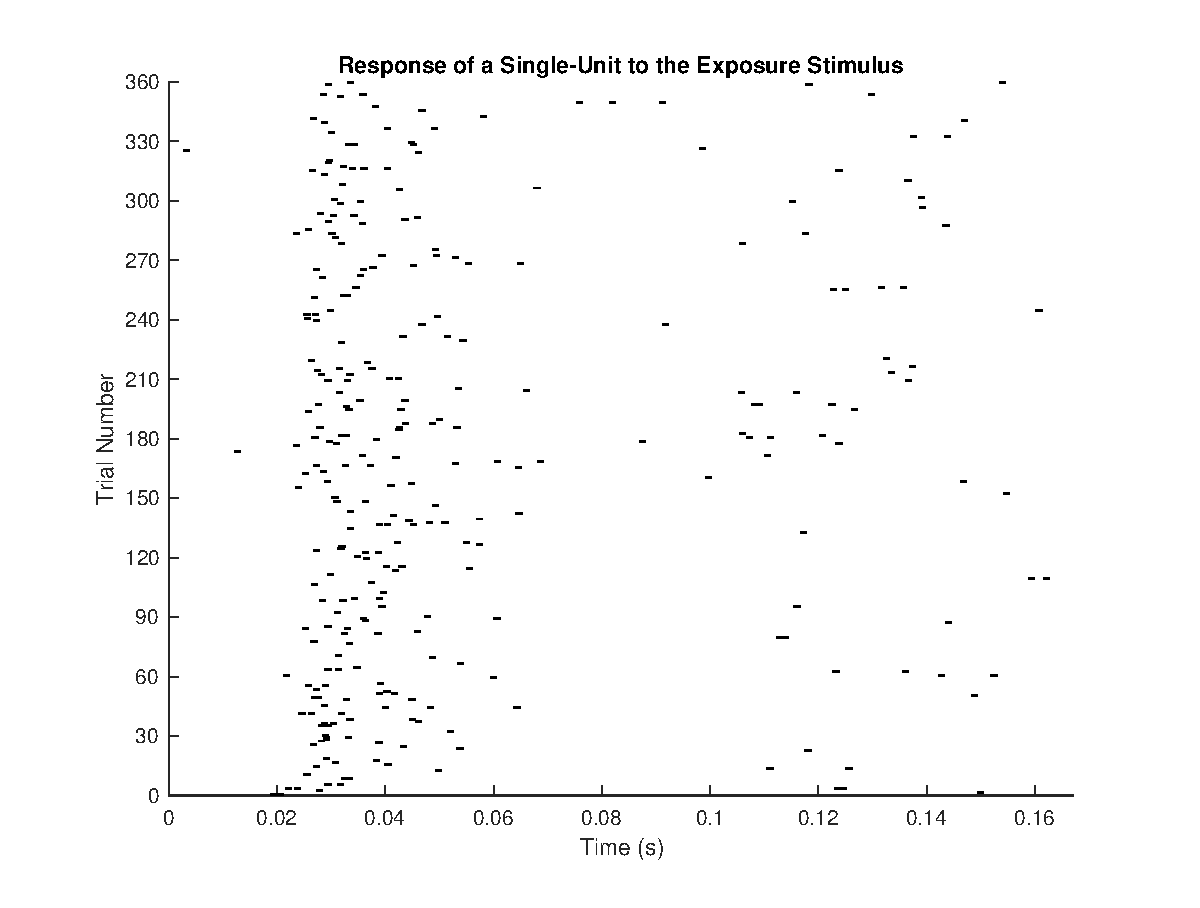
\includegraphics[width=1\textwidth]{RasterPlot.eps}
\caption{Raster Plot of Single-Unit Activity}
\label{fig:RasterPlot}
\end{figure}


\end{document}